%for a more compact document, add the option openany to avoid
%starting all chapters on odd numbered pages
\documentclass[12pt]{cmuthesis}

% This is a template for a CMU thesis.  It is 18 pages without any content :-)
% The source for this is pulled from a variety of sources and people.
% Here's a partial list of people who may or may have not contributed:
%
%        bnoble   = Brian Noble
%        caruana  = Rich Caruana
%        colohan  = Chris Colohan
%        comar    = Cyrus Omar
%        jab      = Justin Boyan
%        josullvn = Joseph O'Sullivan
%        jrs      = Jonathan Shewchuk
%        kosak    = Corey Kosak
%        mjz      = Matt Zekauskas (mattz@cs)
%        pdinda   = Peter Dinda
%        pfr      = Patrick Riley
%        dkoes = David Koes (me)

% My main contribution is putting everything into a single class files and small
% template since I prefer this to some complicated sprawling directory tree with
% makefiles.

% some useful packages
\usepackage{libertine}
\usepackage{fullpage}
\usepackage{graphicx}
\usepackage{amsmath, lipsum, afterpage}
\usepackage[numbers,sort]{natbib}
\usepackage[backref,pageanchor=true,plainpages=false, pdfpagelabels, bookmarks,bookmarksnumbered,
%pdfborder=0 0 0,  %removes outlines around hyper links in online display
]{hyperref}
\usepackage{subcaption}
\usepackage{booktabs}
\usepackage{caption}

\usepackage[capitalize,noabbrev,nameinlink]{cleveref}
\usepackage{float}
\usepackage[scaled]{inconsolata}

\hypersetup{colorlinks,linkcolor={black},citecolor={blue},urlcolor={black}}  

\captionsetup{labelfont=bf}
% \captionsetup{font=small}
\captionsetup{labelfont=bf}
\captionsetup{textfont={}}
%\captionsetup[subfloat]{font=small}
%\captionsetup[subfloat]{farskip=5pt}
%\captionsetup[subfloat]{captionskip=1pt}

\newcommand{\dbSQL}[1]{\texttt{\textbf{#1}}\xspace}

\DeclareUnicodeCharacter{0097}{~}


% Approximately 1" margins, more space on binding side
%\usepackage[letterpaper,twoside,vscale=.8,hscale=.75,nomarginpar]{geometry}
%for general printing (not binding)
\usepackage[letterpaper,twoside,vscale=.8,hscale=.75,nomarginpar,hmarginratio=1:1]{geometry}

% Provides a draft mark at the top of the document. 
% \draftstamp{\today}{DRAFT}

\begin {document} 
\frontmatter

%initialize page style, so contents come out right (see bot) -mjz
\pagestyle{empty}

\title{ %% {\it \huge Thesis Proposal}\\
{\bf Code Generation Recovery Log Replay for In-Memory Database Management Systems}}
\author{Tianlei Pan}
\date{June}
\Year{2021}
\trnumber{CMU-CS-21-131}

\committee{
Andy Pavlo, Chair \\
Wenting Ye \\
}

\support{}
\disclaimer{}

% copyright notice generated automatically from Year and author.
% permission added if \permission{} given.

\keywords{Code Generation, Log Replay, Recovery, query compilation}

\maketitle

\begin{dedication}
\end{dedication}

\pagestyle{plain} % for toc, was empty

%% Obviously, it's probably a good idea to break the various sections of your thesis
%% into different files and input them into this file...

\begin{abstract}
Code generation is an optimization technique for improving query execution throughput by compiling query plans into native code. This technique, however, leads to design challenges for the recovery system of a database management system. The log replay process will be disjoint from the built-in execution engine that has adapted to operate efficiently on compiled code. This leads to the implementation of a separate execution engine to deal with the execution of log records, which can be a huge waste of engineering efforts. To resolve this design conflict between code generation and database recovery, we present a unified approach to support both query execution and log replay in a code-generation-based DBMS. We ask the recovery system to convert log records into compiled code that will be easily accepted by the execution engine. Our results show that while our approach incurs a higher performance overhead compared to using a separate execution engine, it requires much less engineering effort and is superior in index updates.
\end{abstract}

\begin{acknowledgments}
I would like to thank my professor Andy Pavlo for guiding me through my journey at the CMU Database Group. His passion, energy and commitment motivated me to pursue research in database systems in the first place. I will carry on with my life with the valuable lessons that I learned from him. I would also like to thank my peers in the CMU Database Group for working with me and carrying me through my research work. Finally, I want to thank my family for their unwavering support.
\newline

I wish you all the best.
\end{acknowledgments}



\tableofcontents
\listoffigures
\listoftables

\mainmatter

%% Double space document for easy review:
%\renewcommand{\baselinestretch}{1.66}\normalsize

% The other requirements Catherine has:
%
%  - avoid large margins.  She wants the thesis to use fewer pages, 
%    especially if it requires colour printing.
%
%  - The thesis should be formatted for double-sided printing.  This
%    means that all chapters, acknowledgements, table of contents, etc.
%    should start on odd numbered (right facing) pages.
%
%  - You need to use the department standard tech report title page.  I
%    have tried to ensure that the title page here conforms to this
%    standard.
%
%  - Use a nice serif font, such as Times Roman.  Sans serif looks bad.
%
% Other than that, just make it look good...


\chapter{Introduction}
Database management system (DBMS) is a category of software that are responsible for storing data, analyzing data, and interacting with applications. In 1970, E.F. Codd proposed the relational model of data, 

Depending on the use case, a DBMS can focus more on either capturing data or analyzing data. On-line Analytical Processing (OLAP) DBMSs focus on reading, analyzing and aggregating data that is less likely to be modified. On the other hand, On-line Transaction Processing (OLTP) DBMSs support write-heavy transactions that modify the database frequently~\cite{conn05}.

Regardless of the type of a DBMS, both OLTP and OLAP DBMSs are susceptible to failures. The DBMS may shutdown unexpectedly, fail to execute a query, or cease to function due to corrupted data. These failures threaten the integrity of the database and make the DBMS unreliable. Therefore, it is important for a DBMS to distinguish between different kinds of failures in order to develop mechanisms to maintain integrity.

A DBMS can encounter three types of failures: Transaction Failures, System Failures, and Media Failures\cite{theo83}. Transaction Failures are the most common type of DBMS failures. Transaction Failures occur when a transaction fails to commit, either at its own request (e.g., logical errors) or on behalf of the DBMS (e.g., resource unavailability). When a transaction fails, the system needs to react within its lifetime to prevent data inconsistency~\cite{aries}. The DBMS needs to decide whether and how it should undo the changes of the failing transaction. Since a DBMS is running transactions rapidly while its active, Transaction Failures can occur as much as 100 times per minute\cite{theo83}. System Failures occur due to hardware failures (e.g., power outage), operating system faults (e.g., insufficient memory) or DBMS exceptions. Each of these trigger events can cause the DBMS to shutdown unexpectedly and uncontrollably. System Failures occur less frequently compared to Transaction Failures, but take a much longer time for the DBMS to recover. The database needs to pinpoint time of failure and what changes the DBMS failed to record. Media Failures~\cite{sauer17} happen when the underlying storage device of a DBMS fails (e.g., disk head crash, bad sectors). This type of failure causes permanent data loss to the DBMS. The only way for a DBMS to recover from Media Failures is to restore from a secondary backup storage.

To handle different types of failures, a DBMS needs to develop a recovery system that will restart the database correctly in case of failure. A widely adopted recovery system is to combine write-ahead logging during transaction execution with crash recovery that uses redo (install changes to the database) and undo (remove changes from the database) processes, represented by ARIES\cite{malviya14}. The ARIES (Algorithm for Recovery and Isolation Exploiting Semantics)~\cite{aries} protocol is a recovery method developed by IBM in the 1990s. It guarantees database integrity in the fact of Transaction, System and Media Failures~\cite{aries}. In ARIES, the DBMS records transaction modifications in durable log records before the DBMS propagates changes to a database page to disk. During crash recovery, the DBMS applies changes from the log records to the database with redo and undo processes (i.e., log replay) ~\cite{franklin97}.

However, the original ARIES paper focused on disk-based DBMSs. Recently, we have seen a rapidly increasing number of in-memory DBMSs due to technological advancement in semiconductor memory~\cite{gar92}. Many in-memory DBMSs avoid strictly adhering to the ARIES protocol for recovery. This is due to the fact that a lot of the concepts in ARIES no longer apply to in-memory DBMSs. For instance, ARIES uses undo records to revert changes that have been applied to the database. However, undo records are excessive for many in-memory DBMS recovery systems~\cite{noisepage, malviya14, hekaton2013, scuba14, silo_r}. Performance concerns is another reason why in-memory DBMSs stray from the ARIES protocol. Logging requires the DBMS to interact with the disk. Therefore, logging I/O is a major bottleneck for an in-memory DBMS. This prompts in-memory DBMSs to minimize logging traffic~\cite{faeber17}. An example is the recovery of database indexes~\cite{faeber17}. Disk-based DBMSs log updates to index structures (e.g., B+ Tree) that allow faster recovery during log replay~\cite{aries}. In comparison, in-memory DBMSs do not log index updates~\cite{hekaton2013, noisepage, malviya14, silo_r} and choose to reconstruct indexes from scratch during log replay. Despite the differences, many in-memory DBMSs still use some form of logging~\cite{noisepage, malviya14, hekaton2013, silo_r} in their recovery systems.

In addition to changes in recovery systems, in-memory DBMSs adopt various optimization algorithms for their execution engines\cite{kersten18}. These optimizations aim to increase execution throughput by reducing either the number of instructions that a DBMS executes to run a query, or the clock cycles per instruction (CPI)~\cite{boncz05}. Query compilation/code generation is an important optimization technique used by DBMSs to greatly reduce the number of instructions that the CPU needs to execute\cite{kersten18}. During execution, the DBMS breaks down a query into various tasks~\cite{noisepage, neumann11}. To speed up the execution of those tasks, the DBMS can compile them into native code (e.g., C/C++) with an off-shelf compiler\cite{boncz05}. Query compilation leads to faster query execution because it specializes both the data structures (e.g., hash table) and access methods of a DBMS towards execution efficiency~\cite{neumann11}. Moreover, the compiled code can be optimized around locality that increases the chance of a data tuple being propagated between operators in CPU registers\cite{menon17}.

While query compilation succeeds in increasing the execution throughput of a DBMS, it comes with several drawbacks. Implementing a query compilation system requires additional knowledge of compiler systems (e.g., LLVM) and huge amounts of engineering work to translate different execution tasks\cite{kersten18}. The DBMS also generates low-level machine code that is hard to understand and debug~\cite{kersten18}.

Moreover, the DBMS recovery system is isolated from the query compilation execution engine (i.e., a component of a DBMS that is responsible for execution). Most of the query compilation DBMSs we have surveyed~\cite{noisepage, neumann11, paroski16, craig14} have no conduits between their recovery systems and execution pipelines. The recovery system implements its own functionalities to update the database, but some of these functionalities already exist in the execution engine. For instance, we mentioned that in-memory DBMSs rebuild the indexes during log replay. When a redo process install changes on a table, it also retrieves the indexes on that table and update them (index update). However, the execution engine has already implemented this index update functionality. As a result, the DBMS contains two implementations that provide identical functionalities. The number of those functionalities in the recovery system will eventually amount to the scale of a separate execution engine that is built specifically for log replay.

Therefore, if we can find a way to unify a DBMS's recovery system and execution engine, we can drastically reduce engineering overhead. Furthermore, we believe this unification also increases replay efficiency. Unless the rewritten functionalities in the recovery manager are executed as native machine code, they will be less efficient compared to those in the execution engine that uses query compilation. Therefore, if the DBMS allows the recovery system to invoke functionalities within the execution engine, the log replay process should be more efficient.

\section{Contribution}
We present a system design that will extend the execution engine to create custom programs for replaying physical log records. Our design converts log records into a format that the DBMS can compile into native code to be accepted by the execution engine. We will show that our approach removes the need for introducing extra implementations into the recovery system for functionalities that already exist in the execution engine. We will also verify our assumption that by utilizing the code generation execution engine, the DBMS will have increased log replay efficiency.

We implement our approach in NoisePage\cite{noisepage}, a self-driving in-memory DBMS developed at Carnegie Mellon University. NoisePage is built in C++ and uses the PostgreSQL wire protocol for user communication. The DBMS also depends on query compilation for its execution engine. Our experimental results show that while the code generation recovery approach falls short of recovery throughput compared to baseline recovery, it is more efficient in certain areas (e.g., index maintenance, table constraints) and has higher scalabiltiy for a table with a larger number of columns.

We structure the remainder of the thesis as follows. In Chapter 2, we provide more background information on database recovery, code generation, and motivations behind our approach. In Chapter 3, we present the recovery and code generation architecture in NoisePage and how we implemented our approach in this DBMS. In Chapter 4, we evaluate our implementation by comparing it against NoisePage's builtin recovery system. We discuss related works in Chapter 5 and conclude our thesis in Chapter 6.

\chapter{Background}
In this chapter, we discuss more background information on database recovery and code generation. We then explain how the two components interact within a DBMS and what changes need to be made for them to cooperate.

\section{Database Recovery}
A DBMS ensures database integrity by satisfying the following conditions:
\begin{itemize}
    \item \textbf{Durability of Updates}~\cite{agrawal89}: All the changes made by committed transactions are durable.
    \item \textbf{Failure Atomicity}~\cite{franklin97}: None of the changes made by aborted or failed transactions are persisted visible after recovery.
\end{itemize}

Many DBMSs~\cite{noisepage, malviya14, hekaton2013, silo_r, azure, postgres, mysql} combine logging and recovery protocols to preserve these two conditions in case of failure. Logging is the action of storing information about committed transactions on disk, while recovery is the action of restoring the database system into a consistent state.

The DBMS stores logging information in a special data structure called a log record. A log record contains physical changes (e.g., changes made to a specific physical address) performed on the DBMS, or higher-level information (e.g., user-input query). In write-ahead logging \cite{aries}, the DBMS records physical database changes in a log file before the DBMS persists the changes on disk. A transaction is not allowed to commit until the DBMS persists its corresponding log record.

For disk-based DBMSs, a log record in the log file can be either a redo record or an undo record~\cite{aries}. During recovery, a redo record installs the effects of committed transactions, while an undo record removes the effects on incomplete or aborted transactions. In-memory DBMSs, on the other hand, do not persist uncommitted changes on disk~\cite{noisepage, malviya14, hekaton2013, scuba14, silo_r}. This is because disk-based DBMSs generate dirty pages. These are pieces of modified entries in the database that reside in the memory, but have not yet been persisted to disk by the DBMS. However, in-memory DBMSs do not write dirty data to persistent storage~\cite{noisepage, malviya14, hekaton2013, scuba14, silo_r}. Therefore, in-memory DBMSs do not generate dirty pages, nor do they need to keep undo records. As a result, undo records are no longer required for their recovery systems. Moreover, in-memory DBMSs do not need to generate log records for indexes~\cite{faeber17}. During recovery, the DBMS reconstructs the database with redo records reconstructs and create the indexes simultaneously~\cite{malviya14, hekaton2013}. For each redo record, the recovery system finds the table that it modified, then retrieves all of its indexes from the database catalog ((\cref{fig:recovery_index_update}). Finally, for each index, the recovery system either updates it with new values, or remove entries from the index. 

\begin{figure}[t!]
\centering
\centering
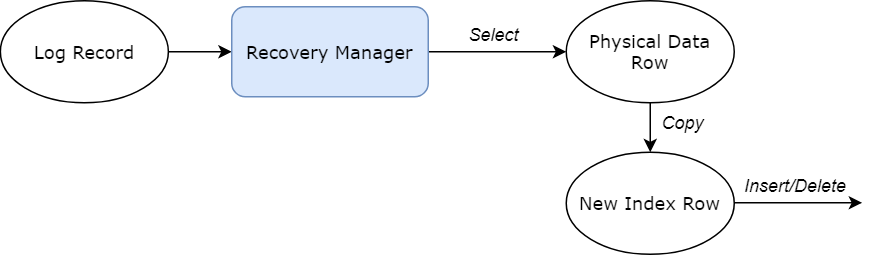
\includegraphics[width=0.9\textwidth]{images/RecoverIndex.png}
\caption{Index Update During Recovery.}
 \label{fig:recovery_index_update}
\end{figure}

\begin{figure}[t!]
\centering
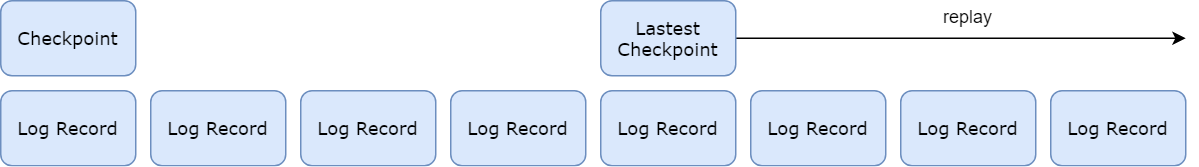
\includegraphics[width=0.9\textwidth]{images/RecoveryCheckpoint.png}
\caption{Recovery with Log Records and Checkpoints.}
\label{fig:recovery_checkpoint}
\end{figure}

Aside from logs, recovery systems can store complete snapshots (i.e., checkpoints) of the database. The DBMS can decide to take checkpoints based on a certain rule (e.g., timed-interval, number of transactions). Checkpoints reduce the time required for the database to recover. The DBMS can directly revert to a previous snapshot without replaying any log records before that snapshot. DBMSs often store both log records and checkpoints. During recovery, the DBMS finds its most recent snapshot, then replays any log records that are stored after that snapshot (\cref{fig:recovery_checkpoint}).

\section{Query Compilation / Code Generation}
\begin{figure}[t!]
\centering
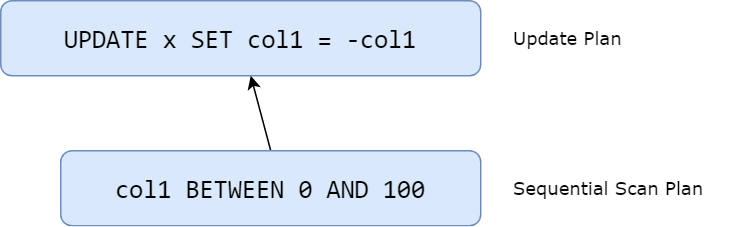
\includegraphics[width=0.5\textwidth]{images/PhysicalPlanExample.png}
\caption{Physical Plan that corresponds to \dbSQL{UPDATE x SET col1 = -col1 WHERE col1 BETWEEN 0 AND 100}.}
\label{fig:physical_plan_example}
\end{figure}
When a query arrives, the DBMS parses the query into an abstract syntax tree (AST). The optimizer of the DBMS then converts the AST into a physical plan tree. The physical plan represents how the DBMS will execute the query. It consists of operators that specify physical operations on the DBMS (e.g., inserting values into a certain memory location). For instance, \dbSQL{UPDATE x SET col1 = -col1 WHERE col1 BETWEEN 0 AND 100} can be represented by an update plan tree with a sequential plan as a child (\cref{fig:physical_plan_example}). The execution engine then uses the plan tree for execution.

In a DBMS that uses query interpretation, its execution engine (i.e., a component of a DBMS that is responsible for execution) processes the physical plan by traversing the plan tree. Therefore, for every query, DBMS needs to follow pointers and resolve branching conditions (e.g., if, switch statements). This incurs overhead caused from virtual function calls, branch mispredictions and instruction cache misses.

\begin{figure}[t!]
\centering
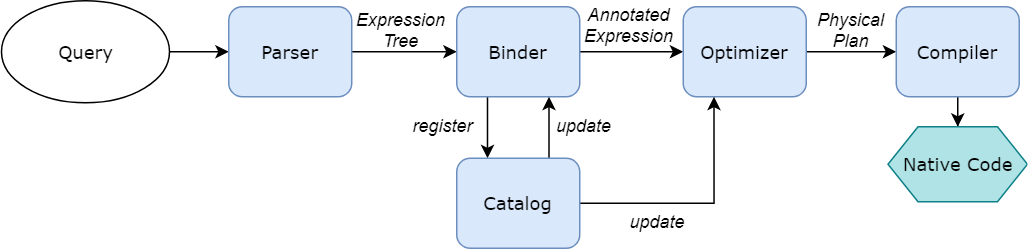
\includegraphics[width=0.9\textwidth]{images/QueryCompilation.png}
\caption{Query Compilation Architecture.}
\label{fig:query_compilation}
\end{figure}

Query compilation eliminates the cost of query interpretation by compiling the physical plan to machine code that is specific for that query. The machine code of the corresponding physical plan can then be executed repeatedly by the execution engine, removing any need for virtual function calls and branching resolutions. Generally, there are two ways of compiling queries. In the first approach, the DBMS creates source code that is compiled into native code with an external compiler (e.g., gcc) ~\cite{krikellas10, klonatos14}. This approach is used in Amazon Redshift and pre-2016 MemSQL~\cite{paroski16}. In the second approach, the DBMS first converts physical plan into an intermediate representation (e.g., LLVM) that follows the grammar of an imperative language. This approach simplifies the process of converting the physical plan into machine code, as the intermediate representation form is designed to resemble SQL statements. Moreover, it removes the need for the DBMS to use the compiler as an external process. This approach is adopted by NoisePage~\cite{menon17}, Hyper~\cite{neumann11}, Hekaton~\cite{craig14}, and SingleStore~\cite{paroski16}.

\section{Motivation}
\begin{figure}[t!]
\centering
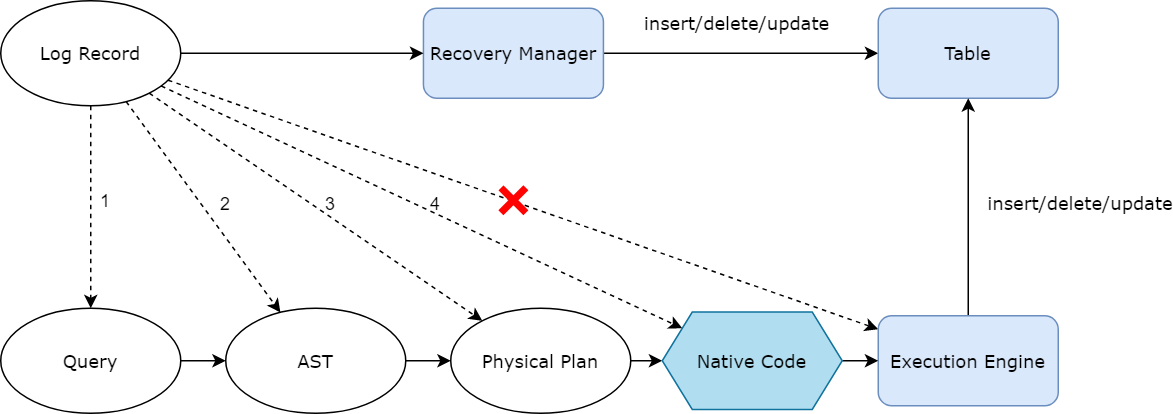
\includegraphics[width=0.9\textwidth]{images/Motivation.png}
\caption{Possible ways to integrate a physical logging system with code generation.}
\label{fig:motivation}
\end{figure}
While code generation is a powerful optimization technique, it poses design challenges for the recovery system. Both the execution engine and physical log records perform identical physical operations on a database table. The native code generated through query compilation operates directly on physical tables. For physical log records, they are already designed as a data structure that represents physical changes made to the database. During recovery, the DBMS simply replays those changes on the table.

However, the recovery system has no means of reusing functions within the execution engine to install physical changes from log records. The execution engine does not accept physical log records because it follows along the query compilation pipeline. This pipeline transforms one logical representation of a query to another, until the query becomes native code. There is no place for physical log records to exist within this transformation pipeline.

There are two solutions to this problem. One solution is to re-implement functions to install physical changes on data tables within the recovery system. However, this approach completely isolates the recovery system from the execution engine. This means that if the recovery system wishes to use a functionality within the execution engine, it has to rewrite that same functionality within the recovery system (\cref{fig:recovery_index_update}).

The other solution is to integrate physical logging with the execution engine. \cref{fig:motivation} shows four possible paths that allow the execution engine to accept physical log records. Converting the log record directly into native code requires the implementation of a new compiling framework, which makes this option infeasible. Therefore, the closest point where the log records can reach before entering the execution engine is physical plans. We then reach the conclusion to convert log records into physical plans. Firstly, compared to raw queries or abstract syntax trees, physical plans are closer to the end of the query compilation pipeline. If we convert a log record into an abstract syntax tree (AST), the DBMS still needs to do additional work to convert the AST into a physical plan. Secondly, we will show in later sections that it is enough for physical plans to represent contents of a log record.

If the DBMS can convert log records into physical plans, the recovery system can rely on code generation for recovery operation. This code generation recovery approach brings around several benefits. Firstly, it significantly reduces engineering overhead. Compiling contents of the log records into machine code allows the recovery system to seamlessly integrate with the built-in execution engine. We have explained in Section 2.1 that the recovery system needs to perform extra operations (e.g. \cref{fig:recovery_index_update}) besides updates to the data tables. These functionalities exist within the execution engine. If we allow the recovery system to reuse existing functionalities by communicating with the execution engine through native code, then the recovery system no longer needs to implement its own functionalities. Secondly, utilizing the code generation execution engine provides more efficient functionalities. A function implemented by the recovery system will not be as efficient as one that exists in the execution engine.

These potential benefits motivate us to design a code generation recovery system based on conversion from log records to physical plans. In the next chapter, we will present the implementation of our approach .

\chapter{Method}
\afterpage{%
\begin{figure}[t!]
\centering
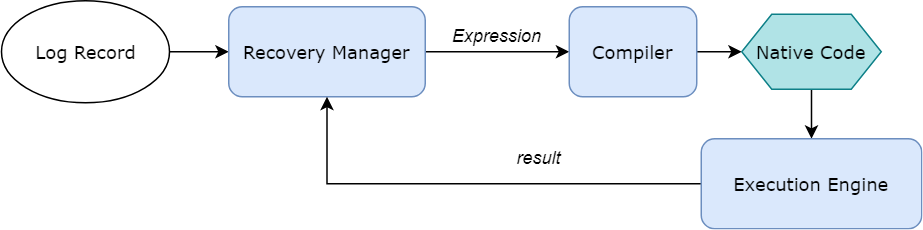
\includegraphics[width=0.9\textwidth]{images/Method.png}
\caption{Code Generation Recovery Mechanism.}
\label{fig:codegen_recovery}
\end{figure}}

We now describe how to extend the recovery system and query compilation pipeline to support log replay with code generation. Our implementation follows along the third option shown in \cref{fig:motivation}. We first enable the recovery system to convert log records into compiled native code. To achieve this, the DBMS needs to interpret the log records into physical plans and prepare them for compilation. We then need to make minor modifications to the execution engine, so it will be able to correctly execute the native code generated by the recovery system. We further summarize our approach (\cref{fig:codegen_recovery}) in two steps:

\begin{enumerate}
\item Convert the log records into physical plans that can be compiled into native code (Recovery Code Generation).
\item Run the compiled machine code using the execution engine (Recovery Execution) for log replay.
\end{enumerate}
We implement our approach in NoisePage~\cite{noisepage}. Noisepage depends on a recovery system that uses physical logging schemes. It also adopts query compilation optimization for its execution engine.

\section{Recovery System Architecture}
 To show how we will extend the recovery system, we first present some background information on the recovery system architecture of NoisePage. NoisePage's recovery system consists of three major components: Transaction Manager, Logging Manager, and Recovery Manager. The Logging Manager interacts with the Transaction Manager to achieve physical logging, while the Recovery Manager interacts with the Transaction Manager to provide database recovery. 

\subsection{Transaction Manager}
The Transaction Manager is responsible for creating and maintaining database transactions. NoisePage uses a transaction to perform physical updates on the database and physical logging to disk. NoisePage uses a multi-versioned delta store~\cite{reed78} Transaction Manager that ensures \texttt{SNAPSHOT-ISOLATION}~\cite{berenson95}. The Transaction Manager allows non-blocking reads over writes and vice versa, but does not allow write-write conflicts on a per tuple basis. A transaction's lifecycle starts when the transaction begins, and ends after the log manager has serialized its changes to disk.

Each data tuple in NoisePage is uniquely identified through a tuple slot that stores the offset of a tuple in a data block. When the DBMS inserts a tuple into a table, it creates a new tuple slot that points to a memory location within the table's data block. Subsequent updates to the tuple does not create direct copies of the tuple, but stores delta information (redo records) about the updates instead. These redo records are essential for executing log replay correctly. The structure of a redo record is shown later in \cref{fig:log_record}.

A transaction uses a buffer (redo buffer) that stores all the delta records that will be generated in its lifetime. Each redo buffer has a fixed size and is allocated from a centralized memory pool. Each time a transaction needs to change the contents of the DBMS, it will attempt to request space from the redo buffer to store a corresponding delta record of the change. If the redo buffer runs out of space, the transaction will replace the current buffer with a new buffer from the memory pool. The redo buffer allows the logging components to process the changes before the transaction ends.

When a transaction commits, the Transaction Manager creates a commit record that contains a timestamp that refers to the oldest active transaction from the timestamp manager. The commit record is appended to the redo buffer. The redo buffer is then carried over to the log manager, where the changes will be serialized to disk. When a transaction aborts, the transaction creates an abort record that prevents corresponding records to be replayed during recovery. Abort records are essential to recovery; since the redo buffer is persisted to disk by the log manager once it is full, it is possible for aborted transactions to persist on disk. During recovery, the DBMS needs to remove aborted transactions. Aborted transactions that are persisted on disk are rare~\cite{tpc15}, however, since it would be difficult for an OLTP transaction to fill up the entire redo buffer.

\subsection{Log Manager}
\begin{figure}[t!]
\centering
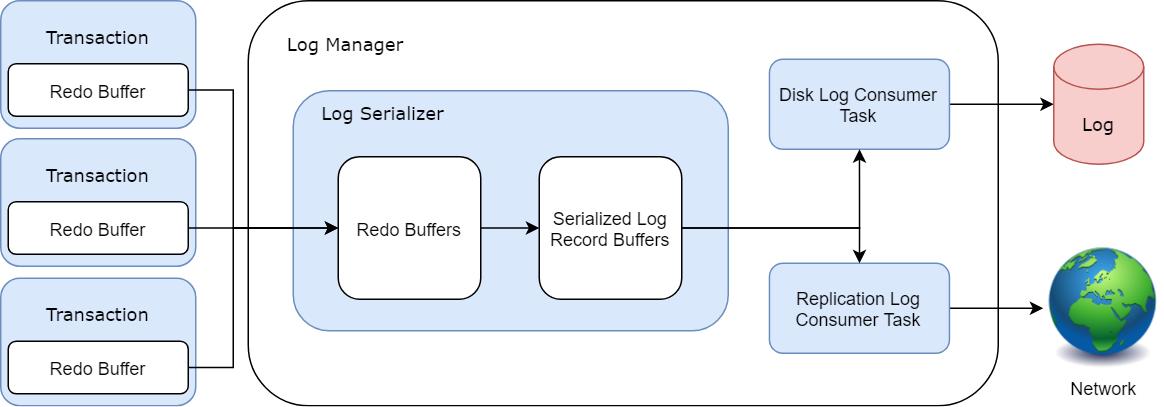
\includegraphics[width=0.9\textwidth]{images/WAL.png}
\caption{\textbf{Log Manager}.}
\label{fig:log_manager}
\end{figure}

The Log Manager (\cref{fig:log_manager}) is responsible for performing write-ahead logging~\cite{aries} in NoisePage. Each log record is self-contained and does not require any additional metadata to be replayed. The Log Manager consists of two separate tasks that live in different threads: the Log Serializer tasks and the Log Consumer tasks.

\subsubsection{Log Serializer}
The Log Serializer task receives redo buffers from a transaction once it is full, or when the transaction decides to commit. The Log Serializer breaks down the redo buffers into raw memory segmented into fixed-size buffers. The Log Consumer consumes these buffers for persistence.

The DBMS must serialize log records in the correct order for recovery to perform correctly. Different transactions can share a same redo buffer that is filled with each of their own log records. Moreover, it is possible for transactions to appear in a non-serial order relative to their begin timestamp. However, the log records performed by an individual transaction is guaranteed to appear in the same order as they were created. This property helps ensure \texttt{SNAPSHOT-ISOLATION} property of NoisePage during log replay.
\subsubsection{Log Consumer}
Different Log Consumers are responsible for consuming buffers supplied by the Log Serializer. The Log Serializer provides each Log Consumer a copy of the original buffer to achieve parallelism. NoisePage uses two type of log consumers: Disk Log Consumer and Replication Log Consumer.

The Disk Log Consumer repeatedly polls for new buffers from the log serializer and writes the changes to disk. To improve performance, disk log consumer uses group commit that allows a batch of changes to be committed over a time period specified by the user. Under default settings, the disk log consumer writes down changes every 10 microseconds of if more than 1 MB of data has been written since the last write.

The Replication Log Consumer also polls for new buffers. Instead of persisting them to disk, it sends the new buffers over across the network to database replicas.

\subsection{Recovery Manager}
\begin{figure}[t!]
\centering
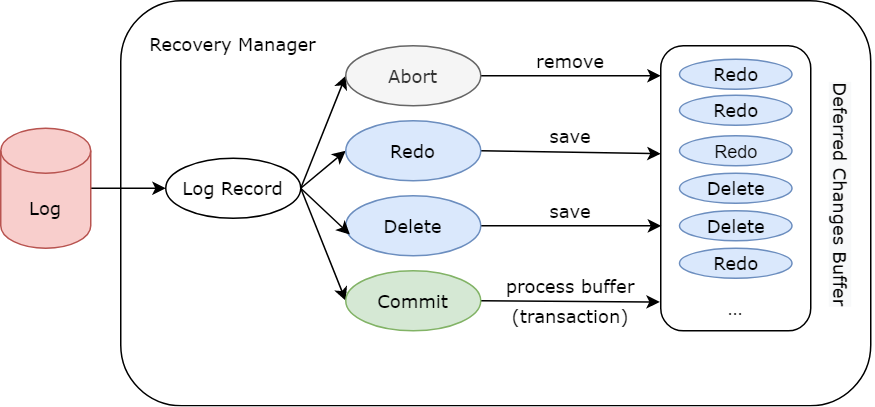
\includegraphics[width=0.9\textwidth]{images/RecoveryManager.png}
\caption{Recovery Manager.}
\label{fig:recovery_manager}
\end{figure}

\cref{fig:recovery_manager} shows the architecture of the Recovery Manager that is responsible for log replay. The Recovery Manager loads the log records into memory and use them to performs log replay. NoisePage uses four different record types: redo, delete, commit, abort. The Recovery Manager do not process redo and delete records are immediately. Instead, the Recovery Manager place redo and delete records inside a deferred changes buffer, ordered by their transaction timestamp. An abort record removes a corresponding redo/delete record from the buffer using the begin transaction timestamp (\cref{fig:log_record}). A commit record initiates a transaction to iterate over the deferred changes buffer. Once all the Recovery Manager processed all the deferred changes, it clears the buffer and commits the transaction. The transaction aborts if any log record is malformed or any replay fails.

\subsubsection{Log Record}
\begin{figure}[t!]
\centering
\begin{subfigure}{.5\textwidth}
 \centering
 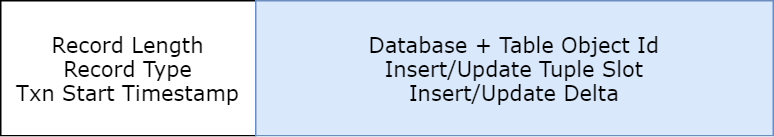
\includegraphics[width=0.9\textwidth]{images/RedoRecord.png}
 \caption{Redo Record Structure.}
  \label{fig:pipeline_graph}
\end{subfigure}%
\begin{subfigure}{.5\textwidth}
 \centering
 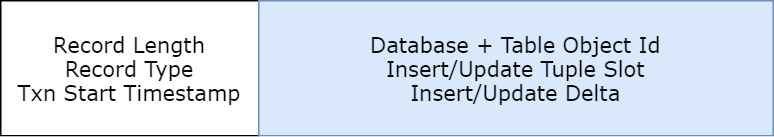
\includegraphics[width=0.9\textwidth]{images/DeleteRecord.png}
 \caption{Delete Record Structure.}
  \label{fig:pipeline_code}
\end{subfigure}
\caption{Log Record.}
\label{fig:log_record}
\end{figure}

A physical log record consists of a header, followed by a record body (\cref{fig:log_record}). The header stores metadata about the log record itself. This includes a log record's record type, size, and begin timestamp of the transaction (See Section 3.1.1). The record body contains physical information that is necessary for recovery and varies depending on the record type. Depending on the value type, the values may bee stored in-line or not in-inline. Simple types such as \texttt{INTEGER}, \texttt{FLOAT} can be stored in-line, while \texttt{VARLEN} entry may store a pointer in the values column that points to another physical location in the record.

Tuple slots in the log records will no longer be valid memory locations during recovery. Instead, the Recovery Manager creates an internal mapping from original tuple slots to new tuple slots that will be retrieved after new values are inserted. The tuple slot mapping allows the Recovery Manager to apply changes to the correct memory locations in the new memory environment.

\begin{figure}[t!]
\centering
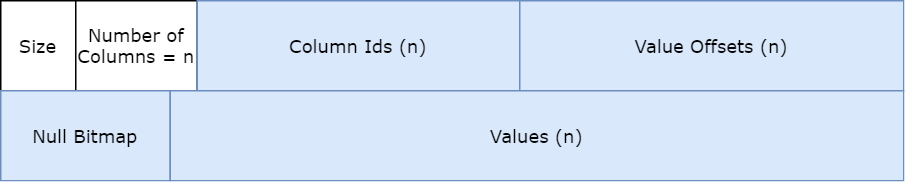
\includegraphics[width=0.9\textwidth]{images/Delta.png}
\caption{Redo Record Projected Row.}
\label{fig:projected_row}
\end{figure}
\begin{figure}[t!]
\centering
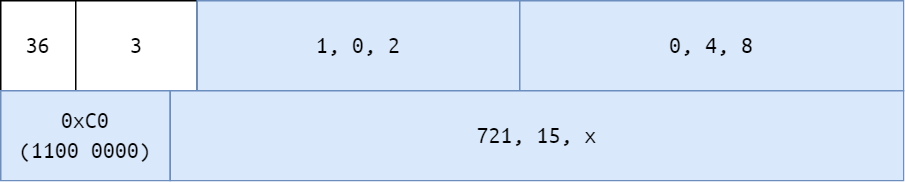
\includegraphics[width=0.9\textwidth]{images/PRExample.png}
\caption{Projected Row that represents [15, 721, \dbSQL{NULL}].}
\label{fig:projected_row_example}
\end{figure}

 While storing tuple slots is sufficient for delete records, redo records require additional data to perform log replay. For instance, to perform an insert, the redo record must contain the values to insert. The Log Manager stores these data in a log record's projected row (\cref{fig:projected_row}). A projected row represents a row in a database table. The DBMS can access an individual value within the projected row by identifying a column id and reading the value using that column's value offset (\cref{fig:projected_row_example}).

\subsubsection{Replay Step}
The Recovery Manager processes each log record differently depending on its record type. Commit and abort records do not change the physical storage of the the database. Therefore, to simplify, we only need to consider the effects of redo and delete records.

We refer to a replay step as the Recovery manager replaying a single redo record or delete record. A NoisePage replay step has three different scenarios:
\begin{itemize}
    \item \textbf{Insert Replay}: The Recovery Manager inserts the values stored within a redo record into the given tuple slot and updates the indexes.
    \item \textbf{Delete Replay}: The Recovery Manager deletes the tuple slot specified by a delete record and updates the indexes.
    \item \textbf{Update Replay}: The Recovery Manager updates the tuple slot using the values within a redo record and updates the indexes.
\end{itemize}

While both insert and update redo records follow the same redo record structure, the Recovery Manager differentiates between them by keeping track of all the tuple slots found in log records. If the Recovery Manager has never seen a tuple slot inside a redo record before, then the redo record represents an Insert operation. Otherwise, the Redo Record represents an Update operation.

\section{Recovery Code Generation}
In this section, we introduce how we integrate the NoisePage's recovery system with its code generation pipeline. We first provide an overview over NoisePage's code generation pipeline. We then show how we convert redo and delete records into physical plans that can be accepted by the code generation pipeline for compilation.

\subsection{Code Generation Pipeline}
The DBMS interprets a query, parses it into an AST and converts it into a physical plan tree. A plan tree consists of plan nodes and specifies how the query should be executed on the physical level of the database.

Code generation is responsible for compiling physical plans into machine code. The code generation pipeline in NoisePage follows from the data-centric compilation approach\cite{neumann11}, as shown in \cref{fig:query_compilation}. The DBMS feeds each plan node into a matching plan translator. Each plan translator correspond to a plan node in the original plan tree. For instance, an insert plan node has a matching insert plan translator; a delete plan node has a matching delete plan translator. A plan translator converts a physical plan tree/node into an operator pipeline. The operator pipeline contains an ordered collection of relational operators (e.g. insert, get table row) that are not yet materialized, ended with a pipeline breaker (e.g., sort tuples, creating a hash table). The execution engine only materializes the pipeline results when a pipeline breaker has been encountered.

\begin{figure}[t!]
\centering
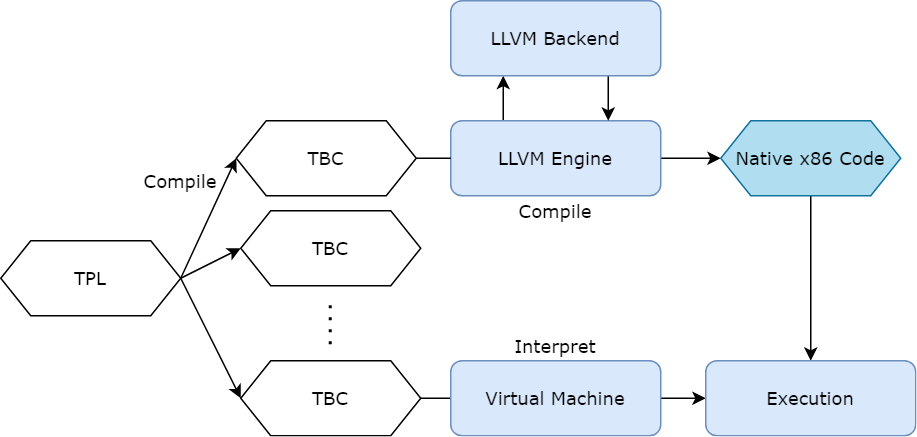
\includegraphics[width=0.9\textwidth]{images/LLVM.png}
\caption{Lifecycle of a TPL code fragment. Execution can run in either interpret or compile mode.}
\label{fig:llvm}
\end{figure}
NoisePage then compiles each operator pipeline into a customized imperative language (TPL). The DBMS then compiles each function of a query inside TPL into some bytecode (TBC). The bytecode can be interpreted by a built-in virtual machine, or further compiled into an LLVM module. The execution engine can either interpret TBC, or run the compiled LLVM module (\cref{fig:llvm}).

\begin{figure}[t!]
\centering
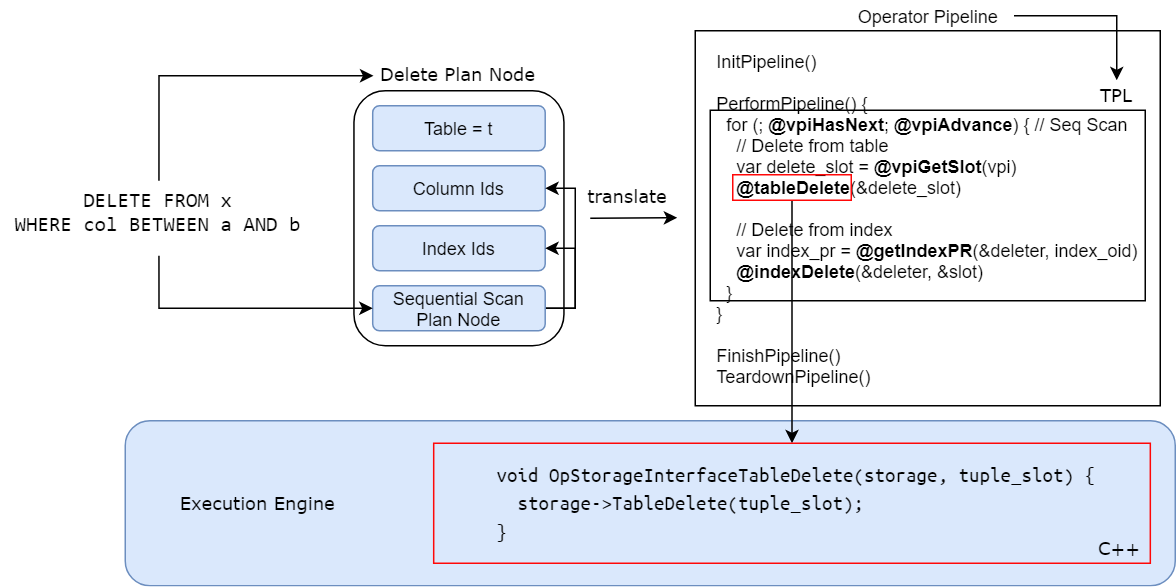
\includegraphics[width=0.9\textwidth]{images/CodegenExample.png}
\caption{Code Generation of \dbSQL{DELETE FROM x WHERE col BETWEEN a AND b}}
\label{fig:codegen_example}
\end{figure}

We further demonstrate the process of query compilation through the example in \cref{fig:codegen_example}. To run the query \dbSQL{DELETE FROM x WHERE col BETWEEN a AND b}, the DBMS needs to first do a sequential scan to find out the columns, then do a delete operation on the found columns. The DBMS represents these two operations in a delete plan node that includes a sequential scan plan node as a child. The DBMS then translates the plan node into an operator pipeline that specifies how each operation will be exactly executed in the DBMS. After this, the DBMS compiles the operator pipeline into machine code (TPL, TBC, LLVM). Each function inside the machine code matches to an operation code function inside the execution engine. When the execution engine runs the compiled code, it invokes its corresponding operation code functions. For instance, \texttt{@tableDelete} corresponds to a C++ function \texttt{OpStorageInterfaceTableDelete} (a delete operation on a tuple slot of a table) in the execution engine.

\subsection{Recovery Integration}
\begin{figure}[t!]
\centering
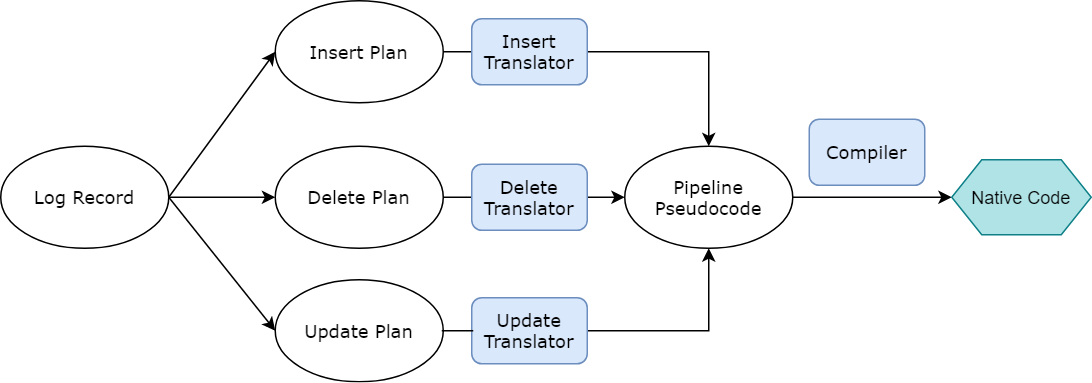
\includegraphics[width=0.9\textwidth]{images/ExpressionGeneration.png}
\caption{Process for converting log records into native code.}
\label{fig:expression_generation}
\end{figure}
We can consider each type of replay as a form of SQL statement that the DBMS can convert into native code through the code generation process discussed above (\cref{fig:expression_generation}). We further divide the code generation process for a log record into three steps: (1) plan generation (creating the physical plan node), (2) plan translation (translating the plan into operator pipelines), and (3) compilation.

In plan generation, the Recovery Manager converts each replay process (insert/update/delete replay) into a corresponding plan node. In plan translation, the Recovery Manager uses matching plan translators to convert physical plans into operator pipelines. Once the Recovery Manager has the operator pipeline, it can then use the compiler to generate machine code for execution.

\subsubsection{Insert Replay Conversion}
\label{insert_replay_conversion}

\begin{figure}[t!]
\centering
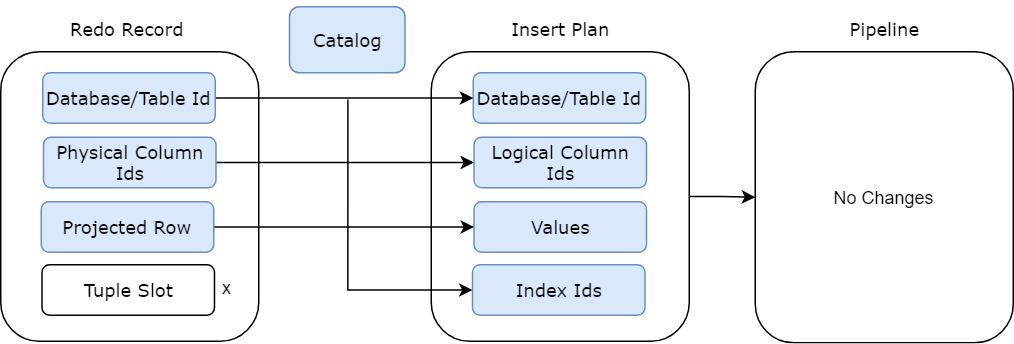
\includegraphics[width=0.9\textwidth]{images/InsertConversion.png}
\caption{Conversion from an Insert Redo Record into an Insert Plan Node. The tuple slot provided by the redo record is discarded.}
\label{fig:insert_conversion}
\end{figure}
Insert plan nodes correspond to \dbSQL{INSERT} statements. We can represent an insert redo record as the SQL statement \dbSQL{INSERT INTO x VALUES y}.

\cref{fig:insert_conversion} shows the conversion from an insert redo record into an insert plan node. The Recovery Manager can retrieve metadata (e.g. table id, column ids) from the redo record and the database catalog. The redo record's projected row contains values for insert (\cref{fig:projected_row}). Those values are in primitive forms (e.g., integer, float, double) as constants. The Recovery Manager then feeds those constants into the insert plan node. This conversion requires no changes to the plan nodes, nor to the operator pipelines.

\subsubsection{Delete Replay Conversion}
\label{delete_replay_conversion}

\begin{figure}[t!]
\centering
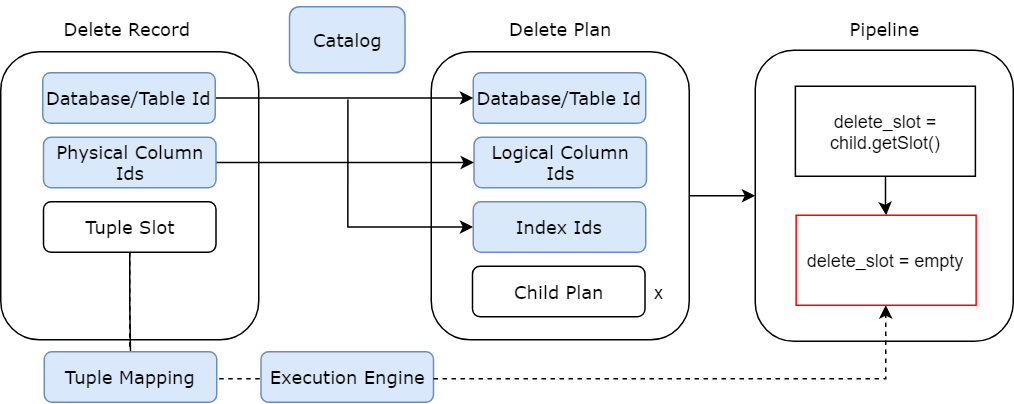
\includegraphics[width=0.9\textwidth]{images/DeleteConversion.png}
\caption{Conversion from a Delete Redo Record into a Delete Plan Node. The operator pipeline uses the tuple slot from the delete record.}
\label{fig:delete_conversion}
\end{figure}

Delete plan nodes correspond to \dbSQL{DELETE} statements. \dbSQL{DELETE} statements require specifications on where the DBMS should perform delete operations (e.g., \dbSQL{WHERE} clause in \cref{fig:codegen_example}). Therefore, a delete plan node requires a child plan node to function. It uses its child plan node to figure out which tuple slot to schedule for deletion.

However, a delete record's tuple slot, combined with the tuple mapping from Recovery Manager, already points to the tuple slot to delete. In this case, there will be no need for the plan node to go through the child node and find out the delete tuple slot. Moreover, delete records do not contain value information that is required for index update (\cref{fig:log_record}). Therefore, we need to provide the operator pipeline with a projected row that contains values that correspond to the row of the tuple slot from the Recovery Manager.

We change the behavior of the operator pipeline as follows (\cref{fig:delete_conversion}): (1) remove the step to look for a new delete tuple slot, (2) retrieve the delete slot supplied by the Recovery Manager during execution, and (3) use the projected row provided by the Recovery Manager for index updates.

\subsubsection{Update Replay Conversion}
\label{update_replay_conversion}

Update plan nodes correspond to \dbSQL{UPDATE} statements. Similar to \dbSQL{DELETE} statements, update plan nodes require child plan nodes. An update operator pipeline expects \dbSQL{SET} clauses returned from the child node (e.g., sequential scan). These \dbSQL{SET} clauses, however, describe higher-level logical operations (i.e., update a column with a certain value). On the other hand, redo records contain low-level physical information (i.e., update a tuple slot with a certain value). Therefore, the Recovery Manager cannot create \dbSQL{SET} clauses efficiently from redo records.

\begin{figure}[t!]
\centering
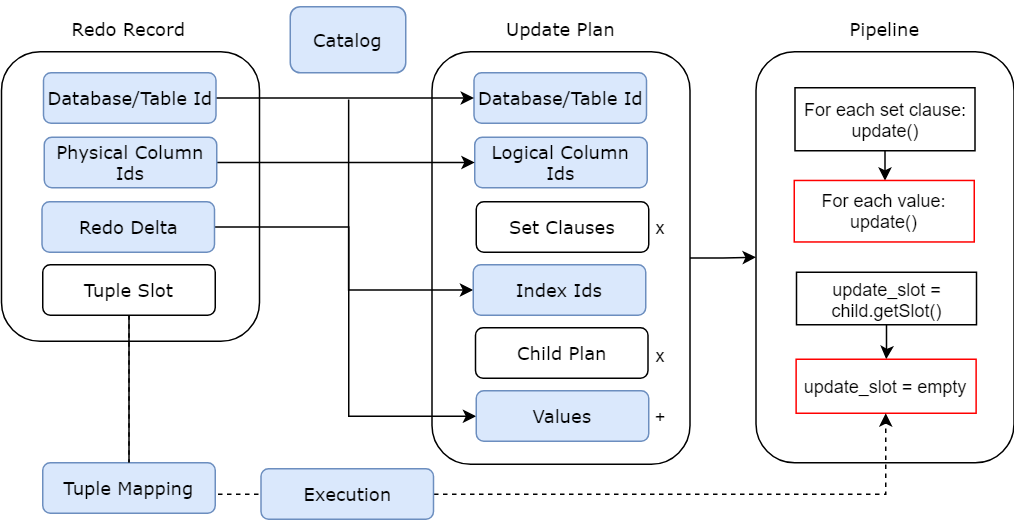
\includegraphics[width=0.9\textwidth]{images/UpdateConversion.png}
\caption{Conversion from an Update Redo Record into an Update Plan Node. \dbSQL{SET} clauses and child plan nodes inside the update plan node are discarded.}
\label{fig:update_conversion}
\end{figure}

We therefore perform the following changes (\cref{fig:update_conversion}): (1) extend the update plan node to accept primitive values like an insert plan node does, (2) modify the operator pipeline to process the primitive values instead of \dbSQL{SET} clauses during a replay step (\cref{fig:update_conversion}), (3) remove the step for update operator pipeline to find out the update tuple slot, and (4) retrieve the update tuple slot from the recovery manager.

\section{Recovery Execution}
We explained in \cref{delete_replay_conversion} that we modified deletes/update operator pipelines to retrieve certain objects (e.g., tuple slots, projected row) from the Recovery Manager. To achieve this, we need to modify the execution engine. The execution engine is responsible for running the compiled query. Inside the execution engine, the compiled query invokes different operation codes (e.g., \texttt{OpStorageInterfaceTableDelete} in \cref{fig:codegen_example}) that correspond to operators in the operator pipeline. Since we modified the operator pipelines earlier, we now need to change operation codes to read in objects from the Recovery Manager.

\subsection{Execution Changes}
\begin{figure}[t!]
\centering
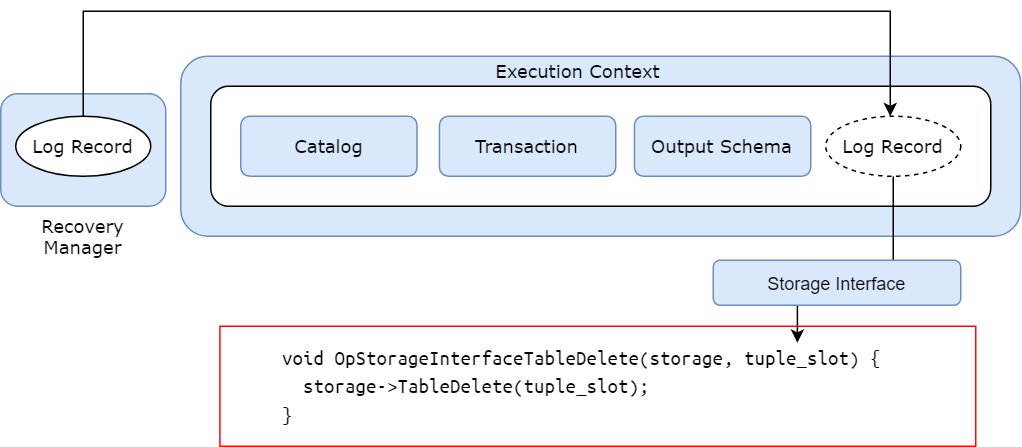
\includegraphics[width=0.9\textwidth]{images/RecoveryExecution.png}
\caption{Operation code functions can access log records through an Execution Context.}
\label{fig:recovery_execution}
\end{figure}
 
We first use the Recovery Manager to set the required tuple slots and projected row into a log record. Before the execution engine runs the query, the Recovery Manager needs to setup a preparation context for execution. In NoisePage, an execution context encapsulates information that is supplied by upper layers of the DBMS (e.g. access to the database catalog, the transaction running the query to execute, database memory pool). We pass the log record from the Recovery Manager into the execution context.

During recovery, for each operation code function that needs to use predetermined tuple slots/projected row for delete/update replays, we enforce it to access those values from the execution context (\cref{fig:recovery_execution}). During the execution of operation codes, NoisePage uses a storage interface object to manipulate over a certain DBMS table. The execution engine initalizes the storage interface object with the execution context. Therefore, the storage interface provides access for the operation codes to access information in the log record from the Recovery Manager.
\section{Caching Optimization}
\label{caching_optimization}

The naive implementation for code generation searches for table metadata and re-compiles the native code every time the Recovery Manager reads in a new log record. This is very inefficient and requires egregious amounts of memory access and copy. We can use caching techniques to reduce this performance overhead.

\subsection{Metadata}
Most of the metadata overhead is generated during the conversion step from a log record into a plan node. For each table, the DBMS needs to figure out its relevant metadata. These operations require frequent lookup into the database catalog. However, all of those metadata are bound to a fixed database and table id. Therefore, the DBMS can cache those metadata with a hash table and re-use them for the same table. Below is a list of important metadata that we have cached successfully:

\subsubsection{Physical to Logical Column Mapping}
The Recovery Manager needs to maintain a mapping from physical column ids to logical column ids for each table. This is required because the column ids recorded in the log records are physical ids, while query compilation expects logical column ids. The Recovery Manager generates this mapping by accessing the database catalog.
\subsubsection{Column Value Type Mapping}
For redo records, the Recovery Manager also needs to maintain a mapping from each column to its corresponding SQL value type (e.g., \dbSQL{INTEGER, FLOAT, VARLEN}). The Recovery Manager uses this mapping to correctly copy the values out of each redo record into an insert/update plan node.
\subsubsection{Catalog Access}
Retrieving access to a database catalog is costly. Profiling results show that a single operation to retrieve catalog access can account for 10\% of total instructions of a replay step. Therefore, the Recovery Manager uses a hash table to keep track of catalog accessors.

\subsection{Compiled Query}
A major benefit of query compilation is that the execution engine can reuse the compiled query. If the contents of a physical plan node remains largely unchanged, then there is no need to reconstruct the physical plan every time the Recovery Manager processes a log record. For instance, we only need to create a new delete plan node if we receive a delete record with a new database and table id.

We can cache each type of replay separately and use a combination of database and table id as unique identifiers. The Recovery Manager can re-use cached queries as long as the table schema associated with them remains unchanged.

\subsubsection{Parameterization}
\begin{figure}[t!]
\centering
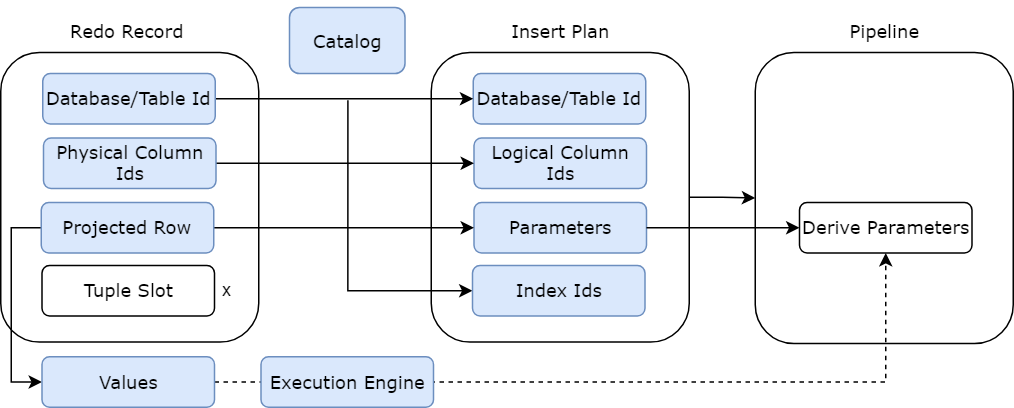
\includegraphics[width=0.9\textwidth]{images/ParameterizedRedoRecord.png}
\caption{Parameterized insert plan.}
\label{fig:parameterization}
\end{figure}

Caching is trickier for replay types that need to transfer values into plan nodes. We mentioned in \cref{insert_replay_conversion} that insert/update needs to copy primitive values from the redo records into plan nodes. In most DBMSs, however, the plan nodes expect primitive values in some wrapper objects~\cite{volcano, kersten18} referred to as expressions. In NoisePage, the corresponding expression for primitive values is a constant value expression. As a result, the Recovery Manager needs to reconstruct a constant value expression for each new value.

A solution to this is to parameterize the constant value expression given to an insert/update plan node. We can represent an insert replay as \dbSQL{INSERT INTO x VALUES @params}. The Recovery Manager caches the plan nodes that contains parameter expressions. The parameters expressions only contain value type information, but do not contain any actual values. During run-time, the execution context passes in primitive values from the Recovery Manager into the plan node.

\chapter{Experimental Evaluation}
We now evaluate the performance of our code generation recovery. The experiments focus on comparing the performance difference between code generation recovery and baseline recovery. Each experiment has two phases: the preparation phase and the recovery phase. During the preparation phase, we use three operations to generate log records: 
\begin{itemize}
    \item \dbSQL{INSERT} $\rightarrow$ \textbf{Insert Redo Record}: Create a random row with random values and insert into a random table.
    \item \dbSQL{UPDATE} $\rightarrow$ \textbf{Update Redo Record}: For a random row from a random table, update a random tuple slot with a random value.
    \item \dbSQL{DELETE} $\rightarrow$ \textbf{Delete Record}: For a random row from a random table, delete a random tuple slot.
\end{itemize}
We run these operations randomly for some number of times during the preparation phase. During the recovery phase, we load the log records into memory from disk and replay them with the Recovery Manager. We then measure the performance of only the replay step in our throughput measurement experiments.

We conduct all the experiments on a machine with the following specifications:
\begin{itemize}
    \item \textbf{OS}: Ubuntu 20.04
    \item \textbf{CPU}: Intel(R) Xeon(R) Gold 5218R CPU @ 2.10GHz
    \item \textbf{RAM}: 188 GB 2 sockets, 20 cores/socket, 40 threads/socket
\end{itemize}

\section{Throughput Measurement}
Log replay generates transactions through commit records (See Section 3.1.2). Therefore, we can use transactions throughput to measure the performance of the recovery phase. 

We use Google Benchmark for our measurement setup. The table starts with an initial table size of $10^6$ tuples. During the preparation phase, we run five preparation operations for each transaction, with a total of $10^5$ transactions. Each table uses a single column and \dbSQL{INTEGER} data type.

\subsection{Insert}
\label{insert_test}

\begin{table}[H]
\begin{center}
\begin{tabular}{ c c c } 
 \toprule
\textbf{Statements Ratio} & \textbf{Baseline Throughput} & \textbf{Codegen Throughput}\\ 
 \toprule
 100\% Insert & $1.12 \times 10^4$ txns/s & $6.00 \times 10^3$ txns/s\\
 \bottomrule
\end{tabular}
\caption{\textbf{Insert Replay Throughput}.}
\label{tab:throughput_exp_insert}
\end{center}
\end{table}
We first measure the throughput (number of transactions executed per time period) of Insert Replays against the baseline recovery performance on a single table. The Recovery Manager uses only our insert replay implementation for recovery.

\begin{table}[H]
\begin{center}
\begin{tabular}{ l c c } 
 \toprule
\textbf{Functionality} & \textbf{IR\%} & \textbf{Normalized IR\%} \\ 
 \toprule
Query Execution (Op Codes) & 79.35 & 81.7\% \\
 \midrule
 Execution Context Initialization & 9.35 & 9.62\%  \\ 
 \midrule
 Retrieving Redo Values & 6.19 & 6.37\%  \\
 \midrule
 Metadata Cache Map Access & 2.26 & 2.32 \%  \\
 \midrule
 Compile & 0.03 & 0.03 \% \\
 \bottomrule
\end{tabular}

\caption{\textbf{Callgrind breakdown on an Insert Replay step}. IR (instructions read) refers to the number of instructions read in total by the selected function during a certain function execution.}
\label{tab:throughput_exp_insert_overhead_all}
\end{center}
\end{table}

\begin{table}[H]
\begin{center}
\resizebox{\columnwidth}{!}{\begin{tabular}{ l c c l } 
 \toprule
\textbf{Operation Code} & \textbf{IR\%} & \textbf{Normalized IR\%} & \textbf{Description}\\ 
 \toprule
\texttt{StorageInterfaceInit} & 29.88 & 74.4\% & Initializes a Storage Interface. \\
 \midrule
\texttt{StorageInterfaceTableInsert} & 6.00 & 14.9\% & Inserts a tuple into a table.\\ 
 \midrule
\texttt{StorageInterfaceFree} & 2.76 & 6.87\% & Deallocates a Storage Interface.\\
 \midrule
\texttt{StorageInterfaceGetTablePR} & 1.40 & 3.48\% & Retrieves a table's projected row.\\
 \midrule
Other & 0.12 & 0.35\% & \\
 \bottomrule
\end{tabular}}
\caption{\textbf{Callgrind breakdown on the Query Execution step of an Insert Replay step}.}
\label{tab:throughput_exp_insert_exec_overhead_all}
\end{center}
\end{table}
Results show that the code generation throughput is 47\% slower than the baseline implementation. Profiling result \cref{tab:throughput_exp_insert_overhead_all} explains that 81.7\% of the slow down comes from the execution of the compiled query. This is unexpected, as we imangined that most of the overhead would come from memory copies for extracting values, but those memory copy overhead only accounts for 6\%.

A further dive into the composition of query execution shows that 74.4\% of the overhead comes from \texttt{StorageInterfaceInit} (\cref{tab:throughput_exp_insert_exec_overhead_all}), which is a function that initializes a storage interface, as explained in Section 3.3. Therefore, the major of overhead of code generation recovery is coming from execution initialization.

\subsection{Delete}
We then measure throughput of Delete Replays against the baseline. The Recovery Manager uses only our delete replay implementation for recovery.
\begin{table}[H]
\begin{center}
\begin{tabular}{ c c c } 
 \toprule
\textbf{Statements Ratio} & \textbf{Baseline Throughput} & \textbf{Codegen Throughput}\\
 \toprule
 90\% Insert, 10\% Delete & $1.12 \times 10^4$ txns/s & $1.08\times 10^4$ txns/s \\ 
 \midrule
 75\% Insert, 25\% Delete & $1.11 \times 10^4$ txns/s & $1.07 \times 10^4$ txns/s\\
 \midrule
 50\% Insert, 50\% Delete & $1.09 \times 10^4$ txns/s & $9.31 \times 10^3$ txns/s\\
 \bottomrule
\end{tabular}
\caption{\textbf{Delete Replay Throughput}.}
\label{tab:throughput_exp_delete}
\end{center}
\end{table}

Code generation throughput results of Delete Replays are much closer to the baseline (90\% to 95\%), compared to those of Insert Replays. This is mainly because a delete operation does not require any memory copies from a redo record. Moreover, executing a delete operation is also a lightweight operation, as we have prevented the pipeline from performing extra work as explained in Section 3.2.2.

\begin{table}[H]
\begin{center}
\begin{tabular}{ l c c l } 
 \toprule
\textbf{Functionality} & \textbf{IR\%} & \textbf{Normalized IR\%}\\ 
 \toprule
Query Execution (Op Codes) & 90.40\% & 91.46\%\\
 \midrule
 Execution Context Initialization & 3.70\% & 3.74\% \\ 
 \midrule
 Delete Record Initialization &4.22\% & 4.27\% \\
 \midrule
 Metadata Cache Map Access & 0.36\% & 0.36\% \\
 \midrule
 Compile & 0.17\% & 0.17\% \\
 \bottomrule
\end{tabular}

\caption{\textbf{Callgrind breakdown on a Delete Replay step}.}
\label{tab:throughput_exp_delete_overhead_all}
\end{center}
\end{table}

\begin{table}[H]
\begin{center}
\resizebox{\columnwidth}{!}{\begin{tabular}{ l c c l } 
 \toprule
\textbf{Operation Code} & \textbf{IR\%} & \textbf{Normalized IR\%} & \textbf{Description}\\ 
 \toprule
\texttt{StorageInterfaceInit} & 24.35 & 76.27\% & Initializes a Storage Interface.\\
 \midrule
 \texttt{StorageInterfaceTableDelete} & 5.80 & 18.16\% & Deletes a tuple from a table.\\ 
 \midrule
 \texttt{StorageInterfaceFree} & 1.55 & 4.85\% & Deallocates a Storage Interface.\\
 \midrule
 Other & 0.13 & 0.41\% & \\
 \midrule
 \texttt{StorageInterfaceGetTablePR} & 0.10 & 0.31\% & Retrieves a table's projected row.\\
 \bottomrule
\end{tabular}}
\caption{\textbf{Callgrind breakdown on the Query Execution step of a Delete Replay step}.}
\label{tab:throughput_exp_delete_exec_overhead_all}
\end{center}
\end{table}

Callgrind results show that (\cref{tab:throughput_exp_delete_overhead_all}, \cref{tab:throughput_exp_delete_exec_overhead_all}), similar to an insert operation, a delete operation is heavily bottlenecked by query execution and initializing the Storage Interface.

\subsection{Update}
Finally, we measure throughput of Update Replays against the baseline. The Recovery Manager uses only our update replay implementation for recovery.
\begin{table}[H]
\begin{center}
\begin{tabular}{ c c c } 
 \toprule
\textbf{Statements Ratio} & \textbf{Baseline Throughput} & \textbf{Codegen Throughput}\\ 
 \toprule
 90\% Insert, 10\% Update & $1.15 \times 10^4$ txns/s & $7.46 \times 10^3$ txns/s\\
 \midrule
 75\% Insert, 25\% Update & $1.15 \times 10^4$ txns/s & $7.31 \times 10^3$ txns/s\\
 \midrule
 50\% Insert, 50\% Update & $1.15 \times 10^4$ txns/s & $6.68 \times 10^3$ txns/s \\ 
 \bottomrule
\end{tabular}
\caption{\textbf{Update Replay Throughput}.}
\label{tab:throughput_exp_update}
\end{center}
\end{table}
The performance of an Update Replay is similar to an Insert Replay. Code generated updates are more heavyweight compared to the baseline insert operations and update operations due to initialization overheads of the Storage Interface. Therefore, as the proportion of update statements increases, we notice a consistent drop on the code generation throughput.

\begin{table}[H]
\begin{center}
\begin{tabular}{ l c c } 
 \toprule
 \textbf{Functionality} & \textbf{IR\%} & \textbf{IR\%/sum(IR\%)} \\ 
 \toprule
Query Execution (Op Codes) & 80.08 & 83.50\% \\
 \midrule
 Execution Context Initialization & 9.41 & 9.81\% \\ 
 \midrule
 Retrieving Record Values & 4.98 & 5.19\% \\
 \midrule
 Metadata Cache Map Access & 1.27 & 1.32 \% \\
 \midrule
 Compile & 0.18 & 0.18 \% \\
 \bottomrule
\end{tabular}

\caption{\textbf{Callgrind breakdown on an Update Replay step}.}
\label{tab:throughput_exp_update_overhead_all}
\end{center}
\end{table}

\begin{table}[H]
\begin{center}
\resizebox{\columnwidth}{!}{\begin{tabular}{ l c c l } 
 \toprule
\textbf{Operation Code} & \textbf{IR\%} & \textbf{IR\%/sum(IR\%)} & \textbf{Description}\\ 
 \toprule
\texttt{StorageInterfaceInit} & 29.84 & 72.50\% & Initializes a Storage Interface.\\
 \midrule
 \texttt{StorageInterfaceTableUpdate} & 8.42 & 20.46\% & Updates a tuple of a table.\\ 
 \midrule
 \texttt{StorageInterfaceFree} & 2.78 & 6.75\% & Deallocates a Storage Interface.\\
 \midrule
 Other & 0.12 & 0.29\% & \\
 \bottomrule
\end{tabular}}
\caption{\textbf{Callgrind breakdown on the Query Execution step of an Update Replay step}.}
\label{tab:throughput_exp_update_exec_overhead_all}
\end{center}
\end{table}

Callgrind results (\cref{tab:throughput_exp_update_overhead_all}, \cref{tab:throughput_exp_update_exec_overhead_all}) show that an update operation is also spending most of its time on query execution and creating the Storage Interface. Combined with results from Section 4.1.1 and 4.1.2, we can confirm that the execution initialization is the main bottleneck of all the code generation recovery.

\section{Index Recovery Throughput Measurement}
\label{insert_index_test}

Most in-memory DBMS do not log indexes to disk~\cite{hekaton2013, noisepage, malviya14, silo_r}. Instead, DBMSs reconstruct indexes during log replay. However, this introduces design problems for an execution engine that has been adapted to work with compiled code. The recovery system needs to implement functionally redundant code to replay the indexes.

In the baseline recovery architecture, the Recovery Manager implements a custom index update function that is independent from the query execution engine. The code generation approach, however, uses the built-in execution engine for index updates. We believe as the number of indexes increases, the performance gap between baseline and the code generation approach will diminish.

\begin{figure}[t!]
\centering
\begin{subfigure}{.45\textwidth}
 \centering
 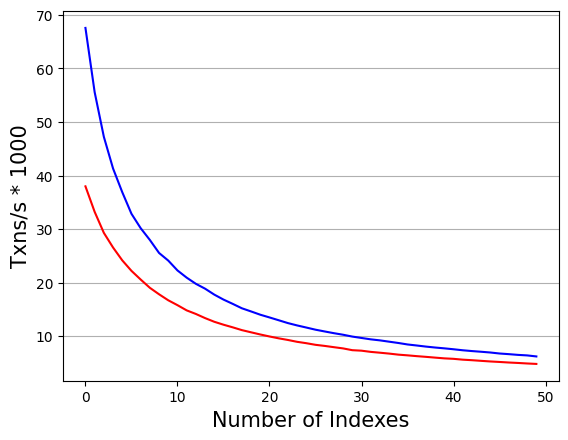
\includegraphics[width=1.0\textwidth]{images/IndexRecoveryThroughput.png}
 \caption{Recovery throughput over the number of indexes. Red is baseline, blue is code generation.}
  \label{fig:index_recovery_throughput}
\end{subfigure}
\begin{subfigure}{.45\textwidth}
 \centering
 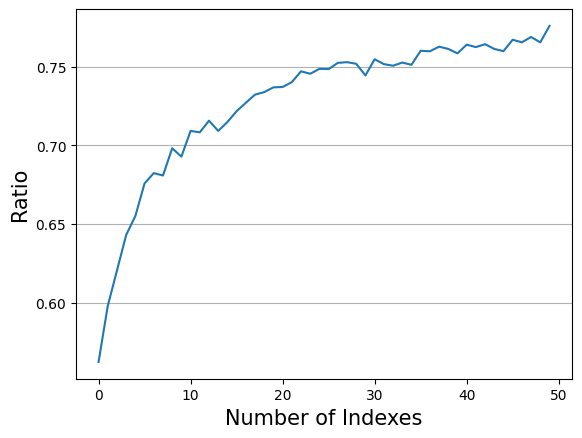
\includegraphics[width=1.0\textwidth]{images/IndexRecoveryRatio.png}
 \caption{Throughput ratio between code generation and baseline implementation.}
  \label{fig:index_recovery_ratio}
\end{subfigure}
\caption{\textbf{Recovery with Indexes}.}
\label{fig:index_recovery_throughput}
\end{figure}

For this experiment, we want to focus on the comparison for index recovery and avoid as much overhead from other operations as possible. Therefore, we go for a much lighter insert setup. However, it should be noted that some of the heavy overhead is still unavoidable (e.g., insert value copies, Storage Interface construction/destruction).

We create an empty table with a single column that accepts \dbSQL{INTEGER} data type. We execute $10^6$ transactions to insert random integers into the table. For each data point, we create an increasing number of indexes for the table. Results show that as the number of indexes increases, the gap between the baseline and code generation implementation steadily decreases. Note that without any indexes, the gap between baseline and code generation is around two times, which matches the results from \cref{tab:throughput_exp_insert}.

\begin{table}[H]
\begin{center}
\begin{tabular}{ l c c } 
 \toprule
\textbf{Functionality} & \textbf{IR\%} & \textbf{Normalized IR\%}\\ 
 \toprule
Index Update & 96.23 & 96.3\% \\
 \midrule
Insert & 3.11 & 3.11\% \\ 
 \midrule
Other (e.g., tuple map access) & 0.57 & 0.59\% \\
 \bottomrule
\end{tabular}
\caption{\textbf{Callgrind breakdown on Baseline Index Recovery}.  Number of indexes is 10.}
\label{tab:throughput_exp_index_overhead_all}
\end{center}
\end{table}

\begin{table}[H]
\begin{center}
\resizebox{\columnwidth}{!}{\begin{tabular}{ l c c l }
 \toprule
\textbf{Operation Code} & \textbf{IR\%} & \textbf{Normalized IR\%} & \textbf{Description}\\ 
 \toprule
\texttt{StorageInterfaceIndexInsertUnique} & 33.77 & 37.9\% & Insert into an index.\\
 \midrule
 \texttt{StorageInterfaceInit} & 32.22 & 36.2\% & Initializes a Storage Interface.\\ 
 \midrule
 \texttt{StorageInertfaceGetIndexPR} & 20.95 & 23.5\% & Retrieves an index's projected row.\\
 \midrule
 \texttt{StorageInterfaceTableInsert} & 1.46 & 1.63\% & Insert a tuple into a table.\\
 \midrule
 \texttt{StorageInterfaceTablFree} & 0.39 & 0.43\% & Deallocates a Storage Interface.\\
 \midrule
 \texttt{StorageInterfaceGetTablePR} & 0.25 & 0.3\% & Retrieves a table's projected row.\\
 \midrule
 Other & 0.02 & 0.02\% &  \\
 \bottomrule
\end{tabular}}
\caption{\textbf{Callgrind breakdown on a Query Execution step of Code Generation Index Recovery}. Number of indexes is 10. The query execution step accounts for 96\% IR for a single replay step.}
\label{tab:throughput_exp_index_exec_overhead_all}
\end{center}
\end{table}

A deeper dive into the implementations shows a percentage difference in index updates between the two approaches. Index updates account for $96.3\%$ of total instructions in the baseline implementation (\cref{tab:throughput_exp_index_overhead_all}). On the other hand, for the code generation approach, index update accounts for $37.9\% + 23.5\% = 61.4\%$ of total instructions (\cref{tab:throughput_exp_index_exec_overhead_all}). This implies that the code generation requires less overhead to prepare for an insert index operation. Therefore, if the DBMS can find a way to mitigate execution initialization overhead, code generation recovery can potentially outperform baseline recovery when the table has high number of indexes.

\section{Throughput Measurement With Scaling Number of Columns}
Our test results with indexes have shown the potential strengths of code generation recovery. Besides indexes, we believe code generation recovery will also be more efficient compared to baseline recovery on a table with a higher number columns. The execution engine has access to more efficient function implementations compared to the Recovery Manager. If we scale the table with higher number of columns, this can potentially reduce the performance gap between the two implementations. To verify our assumption, we performed two tests: (1) An insert recovery test with the same setup as in \cref{insert_test}, and (2) an index recovery test with the same setup in \cref{insert_index_test}.

\begin{figure}[ht!]
\centering
\begin{subfigure}{.44\textwidth}
 \centering
 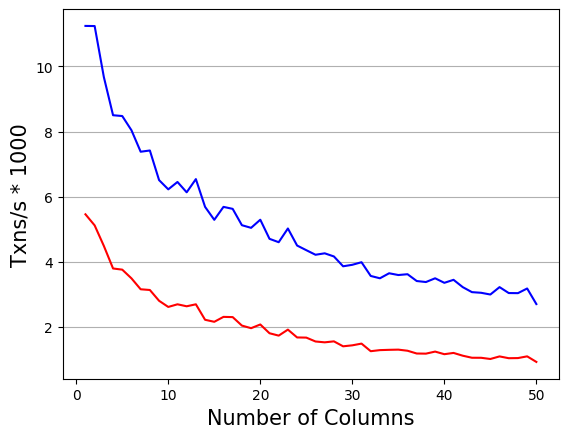
\includegraphics[width=1.0\textwidth]{images/ColumnRecovery.png}
 \caption{Throughput over the number of columns. Red is baseline, blue is code generation.}
  \label{fig:col_recovery_throughput}
\end{subfigure}%
\begin{subfigure}{.45\textwidth}
 \centering
 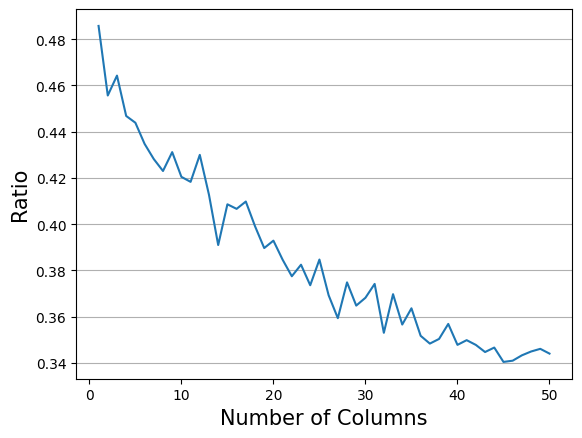
\includegraphics[width=1.0\textwidth]{images/ColumnRecoveryRatio.png}
 \caption{Throughput ratio between code generation and baseline implementation.}
  \label{fig:col_recovery_ratio}
\end{subfigure}
\caption{\textbf{Recovery with Scaling Number of Columns}.}
\label{fig:col_insert_recovery_throughput}
\end{figure}

Results from the insert test (\cref{fig:col_insert_recovery_throughput}) show that code generation recovery failed to shorten the throughput performance gap. Callgrind analysis shows that as the number of columns increase, the execution initialization overhead of code generation also increases. Moreover, a higher number of columns also results in more memory copies for the Recovery Manager to convert an insert redo record int an insert plan node.

\begin{figure}[ht!]
\centering
\begin{subfigure}{.44\textwidth}
 \centering
 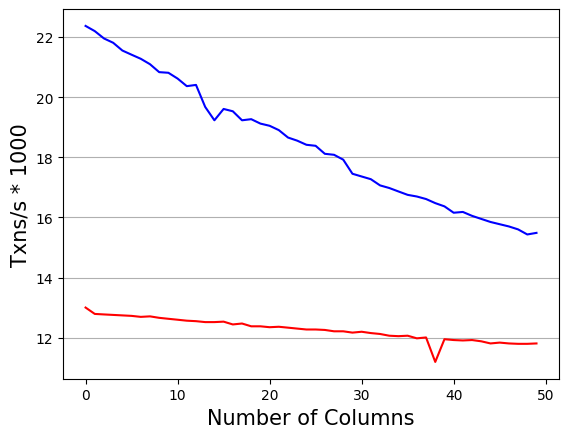
\includegraphics[width=1.0\textwidth]{images/ColumnRecoveryIndex.png}
 \caption{Throughput over the number of columns. Red is baseline, blue is code generation.}
  \label{fig:col_recovery_throughput_index}
\end{subfigure}%
\begin{subfigure}{.45\textwidth}
 \centering
 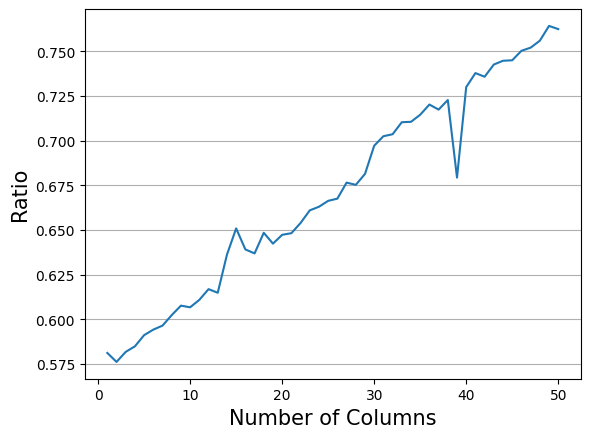
\includegraphics[width=1.0\textwidth]{images/ColumnRecoveryIndexRatio.png}
 \caption{Throughput ratio between code generation and baseline implementation.}
  \label{fig:col_recovery_ratio_index}
\end{subfigure}
\caption{\textbf{Recovery with Scaling Number of Columns}. Number of Indexes is 10. }
\label{fig:col_recovery_throughput_index}
\end{figure}

The index recovery test showed that for index recovery, a higher number of columns have a positive effect in decreasing the gap between code generation recovery and baseline recovery (\cref{fig:col_recovery_throughput_index}). Index recovery has lower execution initialization overhead compared to insert recovery (See \cref{tab:throughput_exp_index_exec_overhead_all}, \cref{tab:throughput_exp_insert_exec_overhead_all}).

\chapter{Related Work}
In this section, we discuss DBMSs with recovery systems that differ from our method assumptions. We then show whether and how our code generation approach applies to them.
\newline

To begin with, our method does not extend to DBMSs that do not have logging architectures. We cannot apply our log record conversion logic to those systems. For instance, Scuba~\cite{scuba14} proposed a recovery system that uses shared memory to persist data between processes. On database shutdown, Scuba copies data directly from memory heap to shared memory. On restart, Scuba retrieves stored DBMS memory from shared memory. This recovery system does not depend on log records, so we cannot apply our approach to such systems.
\newline

Our code generation approach focuses on DBMSs that use physical logging for recovery. However, there are DBMSs that use other logging schemes, such as logical logging and physiological logging~\cite{gray92}. For instance, VoltDB~\cite{malviya14} uses a form of physiological logging known as command logging. The DBMS records transactions instead of physical table changes in the log records. Nevertheless, those log records still correspond to insert, delete, or update operations on the DBMS table. Therefore, we can still apply our log record conversion process to the VoltDB's recovery framework. Hyper~\cite{kemper11} uses logical redo records that keeps the parameters of the stored procedures (i.e. a custom high-level scripting language) that represent the transactions. Hyper uses the stored procedures to provide functionalities such as index, delete, and update. Therefore, we can apply our approach to Hyper by restoring stored procedures using parameters from the log records. We then convert the procedures into respective plan nodes. In fact, converting from logical log records into physical plans might be easier than that for physical log records. According to \cref{insert_replay_conversion}, physical plans expect logical values and data structures (e.g. column ids, \dbSQL{SET} clauses) that can potentially exist directly in logical log records.
\newline

Many in-memory DBMSs also implement parallel recovery to reduce recovery time~\cite{faeber17}. Hekaton~\cite{hekaton2013} uses a thread per core architecture to handle parallel insertion of the data from log records. SiloR~\cite{silo_r} parallelizes recovery by using an epoch system and value logging that allow the recovery system to process log records in arbitrary order. During replay, the recovery system uses multiple log processors to replay log records from newest to oldest. Our code generation recovery approach might introduce extra overhead for parallelization. The recovery system needs to access multiple hash tables (\cref{caching_optimization}) that are necessary for executing compiled queries. This means that with multiple recovery threads, they need to read and modify those hash tables concurrently. All of the hash tables use keys based on database and table ids. Unless the recovery threads manage to operate on separate tables, the recovery system needs to install extra latches on the hash tables. As as result, this incurs performance bottlenecks for parallel recovery.

\chapter{Conclusion and Future Work}
We presented a code generation recovery approach for in-memory DBMSs. Our method integrates the code generation execution engine with the recovery system by converting log records into physical plans and compiling them into native code. We provided an overview of the logging and query compilation architecture of NoisePage. We then showed how we implemented our approach within NoisePage. Finally, we evaluated our approach with throughput experiments. The results show that while code generation recovery has worse recovery throughput compared to NoisePage's baseline recovery, it offers less engineering overhead and is more efficient in processing index updates.

We confirmed that the execution initialization for compiled queries is the main bottleneck for code generation recovery in NoisePage. A possible solution to this is to cache reusable objects that are repeatedly initialized during query execution. We will explore on more solutions to this problem and continue to improve our code generation recovery based on our current implementation in NoisePage. 

%\appendix
%\include{appendix}

\backmatter

%\renewcommand{\baselinestretch}{1.0}\normalsize

% By default \bibsection is \chapter*, but we really want this to show
% up in the table of contents and pdf bookmarks.
\renewcommand{\bibsection}{\chapter{\bibname}}
%\renewcommand{\bibpreamble}{This text goes between the ``Bibliography''
%  header and the actual list of references}
\bibliographystyle{plainnat}
\bibliography{citations} %your bib file

\end{document}
